\documentclass[t]{beamer}

\mode<presentation>
{
  \usetheme{CambridgeUS}  % or try Darmstadt, Madrid, Warsaw, CambridgeUS ...
  \usecolortheme{default} % or try albatross, beaver, crane, ...
  \usefonttheme{default}  % or try serif, structurebold, ...
  \setbeamertemplate{navigation symbols}{}
  \setbeamertemplate{caption}[numbered]
} 

\usepackage[english]{ babel }
\usepackage[utf8x]{ inputenc }
\usepackage{ physics }
\usepackage{ bbold }
\usepackage{ multicol }
\usepackage{caption}
\usepackage{graphicx}
\usepackage{mathtools}


\usepackage{tikz}
\usetikzlibrary{arrows}


\title[Holonomic Optimal Control for Qudits]{Holonomic Optimal Control for Qudits}

\author{ Tomas André}	
\institute{ Uppsala University }

\date{\today}
	
\begin{document}

\begin{frame}
  \titlepage
\end{frame}

%%%%%%%%%%%%%%%%%%%%%%%%%%%%%%%%%%%%%%%%%%%%%%%%%%%%

\section{Introduction}
\begin{frame}
\tableofcontents
\end{frame}

\begin{frame}{Outline}
\tableofcontents[ 
currentsubsection, 
hideothersubsections, 
sectionstyle=show/shaded, 
subsectionstyle=show/shaded, 
] 
\end{frame}

\begin{frame}[c]{Motivation}
''Nature isn't classical, dammit, and if you want to make a simulation of nature, you'd better make it quantum mechanical, and by golly it's a wonderful problem, because it doesn't look so easy.'' 
\\- Richard Feynman
\end{frame}

\begin{frame}{History (1/2)}


\begin{itemize}
\item[1980] Paul Benioff proposes a quantum mechanical model of the turing machine. 
\footnote{{\scriptsize Benioff, Paul (1980). Journal of Statistical Physics.22(5):563.}}


\item[1980s] Both Richard Feynman and Yuri Manin suggests that a quantum based computer could perform calculations not possible on a conventional computer.
\footnote{\scriptsize Feynman, Richard (June 1982). International Journal of Theoretical Physics. 21(6/7):467.}
\footnote{\scriptsize Manin, Yu. I. (1980). Vychislimoe i nevychislimoe [Computable and Noncomputable]}


\item[1994] Peter Shor publishes a quantum algorithm used for finding the prime-factors of an integer.
\footnote{\scriptsize Shor, Peter (1994). IEEE Comput Soc Press:p.124} (This is big!) 


\end{itemize}
\end{frame}

\begin{frame}{History (2/2)}
\begin{itemize}
\item[1998] The first two-qubit quantum computer capable of running calculations is built by Isaac Chaung, Neil Gershenfeld and Mark Kubinec. 
\footnote{\scriptsize Chuang, Isaac L.; Gershenfeld, Neil; Kubinec, Markdoi(1998). Phys. Rev. Lett. American Physical Society. 80(15):3408.}

\item[2019] Google claims to have achieved computations on a quantum machine that would be infeasible on a classical computer.  
\footnote{\scriptsize Gibney, Elizabeth (October 2019). Nature. 574(7779):461.}


\item[Today] Both IBM and Google have active QC research and IBM has a quantum computer with 127 qubits. Despite much focus fault tolerant quantum computers are still a far way off.


\end{itemize}
\end{frame}

\section{Basic Concepts}
\begin{frame}{Outline}
\tableofcontents[ 
currentsubsection, 
hideothersubsections, 
sectionstyle=show/shaded, 
subsectionstyle=show/shaded, 
] 
\end{frame}
\begin{frame}{Quantum Computing}
\textbf{What is Quantum Computing?}


\begin{itemize}
\item Qubits
\item Quantum Gates
\item superposition
\item entanglement 
\item it do be whack yo
\end{itemize}

\end{frame}

\section{Computation from Geometry}

\begin{frame}{Outline}
\tableofcontents[ 
currentsubsection, 
hideothersubsections, 
sectionstyle=show/shaded, 
subsectionstyle=show/shaded, 
] 
\end{frame}


\begin{frame}{What is computation?}

\end{frame}

\begin{frame}{What is computation?}

\begin{figure}
\includegraphics[scale=0.4]{dia1.png}
\end{figure}

\end{frame}


\begin{frame}{What is computation?}

\begin{figure}
\includegraphics[scale=0.4]{dia2.png}
\end{figure}

\end{frame}


\begin{frame}{Computation from Geometry}

\begin{figure}
\begin{center}
\includegraphics[scale=0.25]{geom.png}
\captionsetup{labelformat=empty}
\caption{{\tiny Image credit: Lloyd, Seth (june 2001)."Computation From Geometry". Science vol. 292}}
\end{center}
\end{figure}


\end{frame}



\section{Geometric Quantum Computation}

\begin{frame}{Outline}
\tableofcontents[ 
currentsubsection, 
hideothersubsections, 
sectionstyle=show/shaded, 
subsectionstyle=show/shaded, 
] 
\end{frame}


\begin{frame}{Holonomies (1/2)}

The change of a quantum state is called time-evolution, during one period of time $T$ it is written $U(T,0)$.

The Berry phase is an early example a 1D Holonomy in Quantum mechanics.\footnote{\scriptsize Berry,  (19..)}
\begin{equation}
\ket{\psi(t)} \xrightarrow{\text{time passes}} \ket{\psi(t+T)} = e^{i(\theta + \gamma)}\ket{\psi(t)}
\end{equation}
in this case
\begin{equation}
U(0,T) = e^{i(\theta + \gamma)}
\end{equation}

$\theta$ - dynamical phase, arises from the Hamiltonian of the system.\\
$\gamma$ - 'berry phase', or geometric phase arises from the geometry of the 'landscape'.
\end{frame}

\begin{frame}{Holonomies (2/2)}
More generally the holonomy can be higher dimensional and non-abelian (matrix)
\begin{equation}
U(T,0) = \mathcal{T}\exp\left(i\int_{0}^{T} \underbrace{\mathbf{A}(t)}_{\text{Geometric}} - \underbrace{\mathbf{H}(t)}_{\text{Dynamic}}\,dt\right)
\end{equation}
where $\mathbf{A}_{mn}(t) = i\bra{m(t)}\pdv{}{t}\ket{n(t)}$ and
$\mathbf{H}_{mn}(t) = \bra{m(t)}\mathbf{H}(t)\ket{n(t)}$.
In the non-adiabatic case one wishes to remove dynamical phase contribution, then one is left with the Wilczek-Zee holonomy\footnote{hej };
\begin{equation}
U(T,0) = \mathcal{T}\exp\left(i\int_{0}^{T}\mathbf{A}(t)\,dt\right) = \mathcal{P}\exp\left(i\oint_{C}\mathbf{A}(s)\,ds\right) = U(C)
\end{equation}



\end{frame}


\section{Results}

\begin{frame}{Outline}
\tableofcontents[ 
currentsubsection, 
hideothersubsections, 
sectionstyle=show/shaded, 
subsectionstyle=show/shaded, 
] 
\end{frame}

\subsection{The qutrit}
\begin{frame}{Outline}
\tableofcontents[ 
currentsubsection, 
hideothersubsections, 
sectionstyle=show/shaded, 
subsectionstyle=show/shaded, 
] 
\end{frame}
\begin{frame}{The qutrit}
\textbf{Higher dimensional computational elements?}
\\
Bit: $0$ or $1$ \hspace{1cm} Qubit: $\frac{1}{\sqrt{2}}(\alpha\ket{0} + \ket{1})$



\end{frame}

\begin{frame}{The qutrit}
\textbf{Higher dimensional computational elements?}
\\
bit: $0$ or $1$ \hspace{4cm} qubit: $\frac{1}{\sqrt{2}}(\alpha\ket{0} + \ket{1})$
\\
trit: $0$,$1$, or $2$ \hspace{3.5cm} qutrit: $\frac{1}{\sqrt{3}}(\alpha\ket{0} + \ket{1} + \ket{2})$


\end{frame}

\begin{frame}{The qutrit}
\textbf{Higher dimensional computational elements?}
\\
bit: $0$ or $1$ \hspace{4cm} qubit: $\frac{1}{\sqrt{2}}(\alpha\ket{0} + \beta\ket{1})$
\\
trit: $0$,$1$, or $2$ \hspace{3.5cm} qutrit: $\frac{1}{\sqrt{3}}(\alpha\ket{0} + \beta\ket{1} + \gamma\ket{2})$
\\
$$\mathbf{\vdots} $$
dit $0$,$1$,$\dots$,or $d$ \hspace{3cm} qudit: $\frac{1}{\sqrt{d}}(\alpha\ket{0} + \beta\ket{1} + \dots + \Omega\ket{d})$
\end{frame}

\begin{frame}{The qutrit}
\textbf{Higher dimensional computational elements?}
\\
bit: $0$ or $1$ \hspace{4cm} qubit: $\frac{1}{\sqrt{2}}(\alpha\ket{0} + \beta\ket{1})$
\\
trit: $0$,$1$, or $2$ \hspace{3.5cm} qutrit: $\frac{1}{\sqrt{3}}(\alpha\ket{0} + \beta\ket{1} + \Omega\ket{2})$
\\
$$\mathbf{\vdots} $$
dit $0$,$1$,$\dots$,or $d$ \hspace{3cm} qudit: $\frac{1}{\sqrt{d}}(\alpha\ket{0} + \ket{1} + \dots + \Omega\ket{d})$

\end{frame}


\begin{frame}{The qutrit}
\textbf{Higher dimensional computational elements?}
\\
bit: $0$ or $1$ \hspace{4cm} qubit: $\frac{1}{\sqrt{2}}(\alpha\ket{0} + \beta\ket{1})$
\\
trit: $0$,$1$, or $2$ \hspace{3.5cm} qutrit: $\frac{1}{\sqrt{3}}(\alpha\ket{0} + \beta\ket{1} + \Omega\ket{2})$
\\
$$\mathbf{\vdots} $$
dit $0$,$1$,$\dots$,or $d$ \hspace{3cm} qudit: $\frac{1}{\sqrt{d}}(\alpha\ket{0} + \ket{1} + \dots + \Omega\ket{d})$


\textbf{Pros} and \textbf{Cons}
\begin{itemize}
\item more information per unit
\item operations require fewer gates 
\item harder to control
\end{itemize}
\end{frame}


\begin{frame}{Designing the system}

The idea is the extension of a qubit implemented in a $^{171}$Yb$^{+}$ ion\footnote{Experimental Realization of Nonadiabatic Holonomic
Single-Qubit Quantum Gates with Two Dark Paths in a
Trapped Ion}.
This project is limited to the quantum mechanical models.
\end{frame}


\begin{frame}{Designing the system}
\begin{figure}[H]
    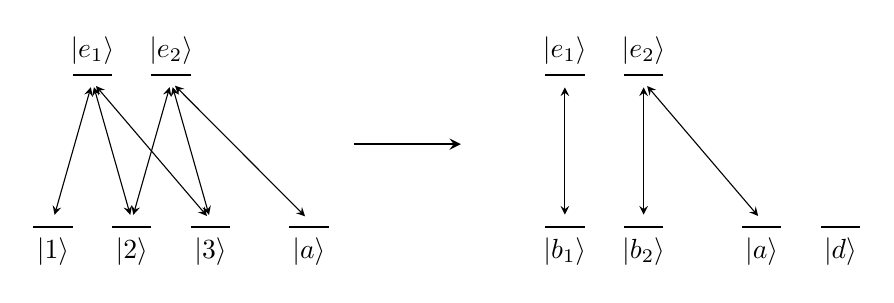
\begin{tikzpicture}[
      scale=0.5,
      level/.style={thick},
      virtual/.style={thick,densely dashed},
      trans/.style={thin,<->,shorten >=2pt,shorten <=2pt,>=stealth},
      arrow/.style={thick,->,shorten >=2pt,shorten <=2pt,>=stealth},
      classical/.style={thin,double,<->,shorten >=4pt,shorten <=4pt,>=stealth}]
      
    % Excited
    \draw[level] (5cm,0em) -- (6cm,0em) node[midway,above] {$\ket{e_1}$};    
    \draw[level] (7cm,0em) -- (8cm,0em) node[midway,above] {$\ket{e_2}$};
	% Ground states
    \draw[level] (4cm,-11em) -- (5cm,-11em) node[midway,below] {$\ket{1}$};
    \draw[level] (6cm,-11em) -- (7cm,-11em) node[midway,below] {$\ket{2}$};
    \draw[level] (8cm,-11em) -- (9cm,-11em) node[midway,below] {$\ket{3}$};
    \draw[level] (10.5cm,-11em) -- (11.5cm,-11em) node[midway,below] {$\ket{a}$};
    % e_1
    % Draw the transitions.
    \draw[trans] (5.5cm,-0.5em) -- (4.5cm,-10.5em) node[midway,left] {};
    \draw[trans] (5.5cm,-0.5em) -- (6.5cm,-10.5em) node[midway,left] {};
    \draw[trans] (5.5cm,-0.5em) -- (8.5cm,-10.5em) node[midway,left] {};
   	% e_2
    \draw[trans] (7.5cm,-0.5em) -- (6.5cm,-10.5em) node[midway,left] {};
    \draw[trans] (7.5cm,-0.5em) -- (8.5cm,-10.5em) node[midway,left] {};
    \draw[trans] (7.5cm,-0.5em) -- (11cm,-10.5em) node[midway,left] {};
    
    \draw[arrow] (12cm,-5em) -- (15cm,-5em) node[] {}; 
    
    % Excited
    \draw[level] (17cm,0em) -- (18cm,0em) node[midway,above] {$\ket{e_1}$};    
    \draw[level] (19cm,0em) -- (20cm,0em) node[midway,above] {$\ket{e_2}$};
    \draw[level] (17cm,-11em) -- (18cm,-11em) node[midway,below] {$\ket{b_1}$};
    \draw[level] (19cm,-11em) -- (20cm,-11em) node[midway,below] {$\ket{b_2}$};
    \draw[level] (22cm,-11em) -- (23cm,-11em) node[midway,below] {$\ket{a}$};
    \draw[level] (24cm,-11em) -- (25cm,-11em) node[midway,below] {$\ket{d}$};
    
  	\draw[trans] (17.5cm,-0.5em) -- (17.5cm,-10.5em) node[midway,left] {};
	\draw[trans] (19.5cm,-0.5em) -- (19.5cm,-10.5em) node[midway,left] {};
	\draw[trans] (19.5cm,-0.5em) -- (22.5cm,-10.5em) node[midway,left] {};
    \end{tikzpicture}    
\end{figure}


\begin{equation}
H = \sum_{j = 1}^2 \sum_{i =j}^{3} \omega_{ij}\ket{i}\bra{e_j}  + \frac{\Omega_{a}(t)}{2}\ket{a}\bra{e_2}  +\,\text{h.c} 
\end{equation}
\begin{equation}
 H_d = \sum_{j = 1}^2 \frac{\Omega_j(t)}{2}e^{-i\phi_j}\ket{b_j}\bra{e_j}  + \frac{\Omega_a(t)}{2}\ket{a}\bra{e_2}  +\,\text{h.c}
\end{equation}

\end{frame}

\begin{frame}{Dark-Bright basis}

The computational basis new computational basis $\{\ket{1},\ket{2},\ket{3}\} \rightarrow \{\ket{d},\ket{b_1},\ket{b_2}\}$ 
parametrized by angles $\theta,\varphi,\chi,\xi$.


\begin{equation}
\begin{aligned}
\ket{d} &= \cos\theta\ket{1} + e^{i\chi}\sin\theta\cos\varphi\ket{2} + e^{i\xi}\sin\theta\sin\varphi\ket{3}
\\
\ket{b_1} &= \frac{1}{\sqrt{1-\sin^2\theta\sin^2\varphi}} \left(-e^{-i\chi}\sin\theta\cos\varphi\ket{1} + \cos\theta\ket{2} \right)
\\
\ket{b_2} &= \frac{1}{\sqrt{1-\sin^2\theta\sin^2\varphi}} \bigg(\frac{1}{2}\sin 2\theta\sin\varphi\ket{1} + \dfrac{e^{i\chi}}{2}\sin^2\theta\sin 2\varphi\ket{2} \\&+ e^{i\xi}(\sin^2\theta\sin^2\varphi - 1)\ket{3}\bigg)
\end{aligned}
\end{equation}

\end{frame}


\begin{frame}{Unitary gate}
\textbf{Constructing the unitary from the basis}
\begin{equation}
\begin{aligned}&
U_1 = \ket{d}\bra{d} -i\ket{e_1}\bra{b_1} -i\ket{e_2}\bra{b_2},\; \phi_1 = \phi_2 = 0
\\&
U_2 = \ket{d}\bra{d} +ie^{i\gamma_1}\ket{b_1}\bra{e_1} +ie^{i\gamma_2}\ket{b_2}\bra{e_2},\; \phi_1 = -\gamma_1,\; \phi_2 = -\gamma_2
\end{aligned}
\end{equation}
\begin{equation}
U(\theta,\varphi,\chi,\xi,\gamma_1,\gamma_2) = U_2U_1 = \ket{d}\bra{d} + e^{i\gamma_1}\ket{b_1}\bra{b_1} + e^{i\gamma_2}\ket{b_2}\bra{b_2}.
\end{equation}
\end{frame}
\begin{frame}{Dark path}



\begin{equation}
\begin{aligned}
\ket{D_1(t)} &= \cos u e^{-i\phi_1}\ket{b_1} + i\sin u \ket{e_1}
\\
\ket{D_2(t)} &= \cos u\cos v e^{-i\phi_2}\ket{b_2} - i\sin u \ket{e_2} - \cos u\sin v \ket{a}
\end{aligned}
\end{equation}
such that $u(0) = u(T) = v(0) = v(T) = 0$

\begin{equation}
\ket{\psi(t)} = f_0\ket{d} + f_1\ket{D_1(t)} + f_2\ket{D_2(t)}, t \in [0,T].
\end{equation}
\end{frame}

\begin{frame}
so for example
\begin{equation}\small
\begin{pmatrix}
1\\
0\\
0
\end{pmatrix}
= f_0 \ket{d} + f_1\ket{D_1(0)} + f_2\ket{D_2(0)} \xrightarrow{t\rightarrow T} \begin{pmatrix}
0\\
1\\
0
\end{pmatrix}
= f_0 \ket{d} + f_1\ket{D_1(T)} + f_2\ket{D_2(T)}
\end{equation}
or equivalent 
\begin{equation}\small
\begin{pmatrix}
1\\
0\\
0
\end{pmatrix}
\rightarrow U\begin{pmatrix}
1\\
0\\
0
\end{pmatrix}
= 
\begin{pmatrix}
0\\
1\\
0
\end{pmatrix}
\end{equation}


\end{frame}

\subsection{Simulation results}
\begin{frame}{Outline}
\tableofcontents[ 
currentsubsection, 
hideothersubsections, 
sectionstyle=show/shaded, 
subsectionstyle=show/shaded, 
] 
\end{frame}

\subsection{Generalization}
\begin{frame}{Generalization}

\end{frame}

\section{Conclusions}

\begin{frame}{Outline}
\tableofcontents[ 
currentsubsection, 
hideothersubsections, 
sectionstyle=show/shaded, 
subsectionstyle=show/shaded, 
] 
\end{frame}
\begin{frame}{Conclusions}

\end{frame}s

\end{document}

